% p3b-02 例2：五角星 五尖角和=180°
\documentclass[tikz,border=4pt]{standalone}
\usepackage{ctex}
\usepackage{amsmath}
\begin{document}
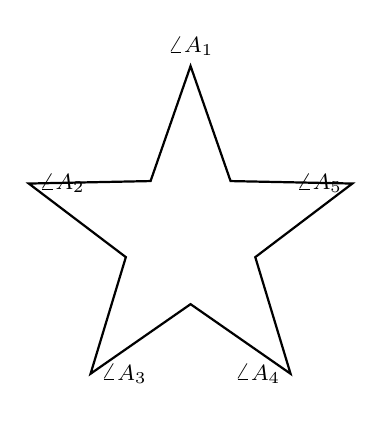
\begin{tikzpicture}[scale=1.2, thick]
  % 5 个外顶点（正五角星）
  \foreach \i in {1,...,5} {
    \coordinate (A\i) at ({90+72*(\i-1)}:1.8);
  }
  % 5 个内顶点（五边形顶点）
  \foreach \i in {1,...,5} {
    \coordinate (P\i) at ({90+36+72*(\i-1)}:0.72);
  }
  % 画五角星：A1-P1-A2-P2-A3-P3-A4-P4-A5-P5-A1
  \draw (A1)--(P1)--(A2)--(P2)--(A3)--(P3)--(A4)--(P4)--(A5)--(P5)--cycle;

  % 五尖标记
  \node[above] at (A1) {\footnotesize $\angle A_1$};
  \node[right] at (A2) {\footnotesize $\angle A_2$};
  \node[right] at (A3) {\footnotesize $\angle A_3$};
  \node[left]  at (A4) {\footnotesize $\angle A_4$};
  \node[left]  at (A5) {\footnotesize $\angle A_5$};
\end{tikzpicture}
\end{document}
